\chapter{Component Tree}\label{chapter:cptree}
Componet tree is one of the main topic in my thesis for cell tracking. In my cell tracking algorithm, each image is converted into a component tree. Then the component trees are used in tree assignment for cell association. Najman and Couprie \cite{Najman:04,najman2006building} proposed a fast way, which is based on Tarjan's union-find procedure, to build a component tree. However, the constructed component tree is usually very large, which is too large for later tree assignment step. It is observed that most nodes in the component tree are redundent which make the tree really big. In this thesis, I proposed a pruning method which decrease the final tree significantly (0.1\% of the original size).\\
Before component tree assignment, we need to compute the weights between every pair of nodes in two component trees. This step is extremely time consuming, which is once a bottle neck of our cell tracking algorithm. However, we proposed a fast dynamic algorithm which enables a quasi-linear running time from $O(|T1|\cdot|T2|\cdot N)$ to $O(N)$.
\section{Component tree construction}
\subsection{Component tree definition}
\subsection{The $\alpha$ and $\beta$ area}
\subsection{Disjoint-set data structure}
\subsection{Quasi-linear algorithm}
\section{Component tree pruning}
Each image is uniquely mapped to a component tree, and vice versa. Usually the constructed component tree is extremly large (133187 nodes for an 8bit image of size 156x250x34). But the tree assignment step only tolerant a tree of size about 200. It is absolutly necessary to prune the component tree before moving into next step.\\
To make the concept clear, the component tree constructed from an image without pruning is called a complete component tree.
\subsection{Redundancy rate}
The redundancy rate of a component tree is defined as the ratio between the size of component tree and that of its corresponding image. For an image of size $N$. The maximum redundancy rate is 100\% when each pixel maps to a component node. The minimum redundancy rate is $1/N$ when there is only one node in the tree with the pixels of the whole image. For the example above, 133187 nodes for an image of size 156x250x34, the redundancy rate is 10.04\%.\\
The redundancy rate reflects the structure complexity of an image. High redundancy indicates an nosiy image with many small components, whereas low rendundancy indicate a clear image with small components. 
\subsection{The redundant nodes}
Fortunately, we find lots of redundant nodes from the statistic of a complete component tree. There are plenty of nodes with very few pixels and huge number of single nodes, which is the only child of its parent. Look at fig\ref{fig:cptree-random}, it is the complete component tree of a random image of size only 10x10, but 79 nodes. The small nodes leads to lots of leaf nodes in the tree. The single nodes contribute most nodes for the tree and make the tree extremly long with high depth. \\
The small nodes usually means a noise component, which should be deleted without hesitation. The single node is created in the instance that when the threshold increase, a big component shrinks to a smaller compoent (the created single node) without breaking into pieces. A path with long single nodes from ancestral node to child node represents the size decreasing tendency of a big ancestral node. The single node without too much change from its parent is not very important and should be deleted.\\
Besides the two main kinds of redundant, there is a third kind of redundant nodes, that is the components with huger size which is more than the object size. 
\begin{figure}[htbp]
\centering
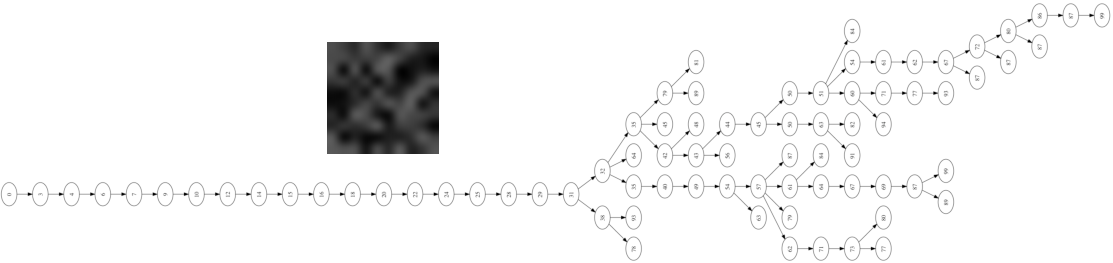
\includegraphics[width=1.0\textwidth]{images/cptree_random}
\caption{The complete component tree of a random image of size 10x10 with 79 nodes (redundancy rate 79\%), there are lots of single nodes in the tree}
\label{fig:cptree-random}
\end{figure}

\subsection{The pruning precedure}
As analysised in above, the nodes with small number of pixels and the single nodes with small changes should be deleted. For the first scenario, the total number pixels of a node is the number of pixels in its $\alpha$ area, named $\alpha$ size. We can set a small $\alpha$ size threshold to filter out these redundancy. For the second scenario, the changing of a single node from its parent is the $\beta$ area of its parent node. Similarly, a small $\beta$ size threshold is set to prevent the parent nodes from creating new single child nodes.\\
Take the same example as before, 
\section{Weights between component trees}
When segment an image with various threshold values, the resulting connected components can be ordered hierarchically as a tree which we call it component tree. Fig. \ref{fig:ct3d-ct1d} shows the component tree (right) of the grayscale (left). It follows the steps, firstly choose many different threshold values to segment the images, which will get a lot of connected components. Then we order the connected component according to their inclusion relationship. Obvious the relationship of these connected components can be represented as a tree.\\
\textbf{Component node}: Each node in the tree is exactly mapped to a connected component, but they are different sets. The connected component is the set of points with intensity larger than a certain value $\theta(0 \sim 255)$. But the node is the set of points in the connected component exclude by either of its child nodes. So the union of the node and its children is equal to its connected component. And the union of all the node is the whole image. \\
\textbf{Terminology}: The threshold value $\theta$ for a connected component is called \textbf{level} in the corresponding node, denoted as $l$. The level of the root node of is always 0. We will refer the \textbf{size} of a node as the number of points it contains and \textbf{total size} of a node as the the number of points in its connected component.
\textbf{Quasi Linear Algorithm}
Currently component tree can be constructed in quasi-linear time \cite{najman2006building}, which is the fastest algorithm now. The time complexity is independent of the number of threshold values. The speed of  building the component tree for 8-bit and 16-bit image has no much difference.\\
\textbf{Disjoint Set Data Structure}: The key technology of this algorithm is due to the usage of disjoint sets data structure \cite{disjointset2006impl} \cite{lect10disjointset}, which is a very efficient data structure to union sets and find the root (reprent the set) of an element.\\
\textbf{Component Tree Pruning}: Although the quasi-linear algorithm is really very fast, we can improve the algorithm even better  by introducing three parameters. The first parameter is minimum size thresholding value denoted as $m$, which means the node with \textit{total size} less than $m$ will be neglected. The second parameter is maximum size thresholding value $M$,  which means  the node with \textit{total size} larger than $M$ will be neglected. The third parameter is single size cut off denoted as $s$, which means the node with only one child, will be neglected if it's \textit{size} is less than $s$. The filtering of the three parameters is called \textit{Component Tree Pruning}. However, the pruning process is not limited to the three parameters. \\
The pruning process needs an operation \textbf{merge to}. Merge node $a$ to node $b$ means put all points of node $a$ into node $b$ and add all children of a to the children of $b$, then delete node $a$ from the tree. \\
For a component tree the pruning order of the three parameter is $m$, $M$, $s$. The first step is minimum size $m$ and maximum $M$ thresholding for each node. The node with \textit{total size} less than $m$ or larger than $M$ will be merged to its parent node. The second step is single node cutoff $s$ thresholding for each node in the tree. The single node with \textit{size} less than $s$ will merge its child to itself.  Fig. \ref{fig:ct3d-clustering} shows two instances of tree pruning process. Each node in the figure is represent by the node \textit{size} and its \textit{total size}. In figure 3-A node (6,6) and (71,71) is merged to their parent then single node (4, 15) meger its child (11,11) to itself. In figure 3-B, only nodes (6,6) and (71,71) are merged to their parent nodes, no other node is merged. However if $s$ is set to 11, node (11,11) will be merged.\\
\textbf{Basic Data Structure}: We will define a minimum component tree data structure, which meet the requirement of tree building algorithm \cite{najman2006building}. The data structure can be expand according to the requirement of programming. We try to make the data structure as clean and clear as possible.\\
\textbf{Clustering Process}: The process of build component tree can be considered as clustering of image points. Points with intensity larger than threshold $\theta$ and connected to each other will be clustered together. Through decreasing of the threshold $\theta$, the cluster will merge its surrounding points into a new cluster. Our clustering process is a little different from traditional binary clustering method which clusters only two components each time. Instead we are not restricted to the number of component in each clustering step. Figure 2 illustrate the difference between binary clustering and multiple clustering. Figure 2-A is the normal clustering process. Figure 2-B is the process of our tree building. From the clustering process we can get some interesting features.
\begin{enumerate} 
	\item If all leaf nodes are omitted, the remaining clusters exactly represent our component tree. Each cluster maps to a node in component tree, each node is the set of leafs which belong to the corresponding cluster. 
	\item From bottom up, the clustering order is from hight intensity points to low intensity points. So the first step of clustering is to sort image points according to their intensity.
\end{enumerate} 
So we can now give out a general description of the clustering process. 

\begin{algorithm}
\SetAlgoLined
\KwData{Image points with various intensity}
\KwResult{The hierarchy  representation of these points}
Sort the points in decreasing order of their intensity.
Create a cluster for each point\\
for each point $p$\\
	find its topmost cluster $c(p)$ \\
	for each neighbor $q$ of $p$ with intensity no less than $p$\\
		find the topmost cluster of $q$ as $c(q)$\\ 
		if $p$ and $q$ have the same intensity , merge $c(p)$ and  $c(q)$ \\
		else 
\caption{Component tree clustering process}
\label{alg:ct3d-clustering}
\end{algorithm}

\begin{figure}[htbp]
\centering
\includegraphics[width=1.0\textwidth]{images/ct3d_ct1d}
\caption{Segmentation of the grayscale image with different threshold values, the segmented connected component is hierarchically ordered}
\label{fig:ct3d-ct1d}
\end{figure}

\begin{figure}[htbp]
\centering
\includegraphics[width=15cm]{images/ct3d_ct_pruning}
\caption{Component Tree Pruning}
\label{fig:ct3d-ct-pruning}
\end{figure}


\begin{figure}[htbp]
\centering
\includegraphics[width=15cm]{images/ct3d_clustering.pdf}
\caption{Component Clustering Processing}
\label{fig:aa}
\end{figure}
